
\section{Data Models, Schemas, and Instances}

A \textbf{client module} handles user interaction and provides user-friendly interfaces. Whereas a \textbf{server module} handles data storage, access, search and other functions.\\

Databases provide \textbf{data abstraction} (suppression of details of data organization and storage and highlighting of essential features). A \textbf{data model} is a collection of concepts that can be used to describe the structure of a database. They also include a set of \textbf{basic operations}.\\

The \textbf{dynamic aspect} or \textbf{behavior} is a set of user-defined operations that are allowed on the database objects (for example compute GPA).\\

\subsection{Categories of Data Models}

\textbf{High-level} or \textbf{conceptual data models} provide concepts that are close to the way many users perceive data. \textbf{Low-level} or \textbf{physical data models} provide concepts that describe the details of how data is stored.\\

Conceptual data models use different concepts:\\

\begin{itemize}
    \item \textbf{Entity}: represents a real-world object or concept (such as an employee or project)
    \item \textbf{Attribute}: represents some property of interest that further describes the entity
    \item \textbf{Relationships}: represents association among the entities. 
\end{itemize}

\subsection{Schemas, Instances, and Database State}

The \textbf{database schema} is the description of the database. It is specified during database design and is not expected to change frequently. A \textbf{schema diagram} is a displayed schema of the database.\\

The database state at a particular moment in time is called a \textbf{database state} or \textbf{snapshot}. 

\section{Three-schema architecture and data independence}

This kind of schema helps to achieve the three following characteristics:\\

\begin{itemize}
    \item Use of a catalog to store the database schema and make it self-describing
    \item Insulation of programs and data
    \item Support of multiple user views
\end{itemize}

\subsection{The three-schema architecture}

The goal is to separate the user applications from the physical database. Schemas can be defined at the following three levels:\\

\begin{figure}[!h]
    \centering
    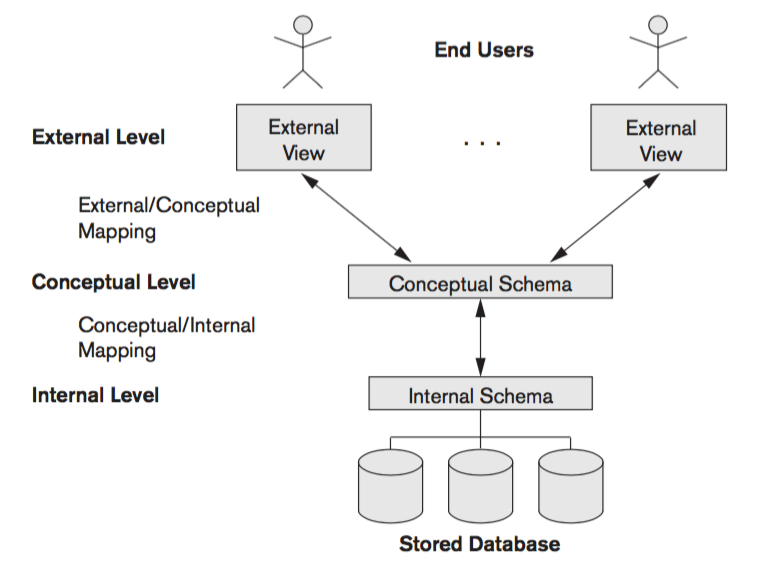
\includegraphics[scale=0.4]{chap2-1.png}
    \caption{Three schema architecture}
    \label{fig:architecture-2}
\end{figure}

\begin{itemize}
    \item \textbf{The internal level} has an \textbf{internal schema} which describes the physical storage structure of the database. It describes the complete details of data storage and access paths.
    \item \textbf{The conceptual level} describes the structure of the whole database for a community of users. It hides the details of physical storage structures and focus on describing entities, attributes, relationships, user operations and constraints.
    \item \textbf{The external or view level} includes a number of external schemas. They describe the views of different user groups.
\end{itemize}

In this architecture, each user group refers to its own external schema. The DBMS must transform a request specified on an external schema into a request against the conceptual schema, and then into a request on the internal schema. When the data is extracted, it must be reformatted to match the user's external view. The processes of transforming requests and results between levels are called \textbf{mappings}.

\subsection{Data independence}

\textbf{Data independence} is the capacity to change the schema at one level without having to change it at the next higher level. There are two types of data independence:\\

\begin{itemize}
    \item \textbf{Logical data independence}: capacity to change the conceptual schema without having to change external schemas or application programs. Only the view definitions and the mappings need to be changed.
    \item \textbf{Physical data independence}: capacity to change the internal schema without having to change the conceptual schema (exact location of data on disk, and hardware details of storage encoding, placement, compression, splitting, merging of records) 
\end{itemize}

Logical data independence is harder to achieve because it allows structural and constraint changes without affecting application programs.

\section{Database languages and interfaces}

\subsection{DBMS languages}

\textbf{Types of languages}:\\

\begin{itemize}
    \item \textbf{Data Definition Language}: used to define both the conceptual and internal schemas
    \item \textbf{Storage Definition Language} : used to specify the internal schema
    \item \textbf{View Definition Language}: used to specify user views and their mappings to the conceptual schema
    \item \textbf{Data Manipulation Language}: used for retrieval, insertion, deletion and update
\end{itemize}

However in current DBMS those languages aren't considered distinct. SQL is a combination of DDL, VDL and DML.\\

There are two types of DML:\\

\begin{itemize}
    \item \textbf{High level} or \textbf{non procedural}: used on its own to specify complex database operations concisely. They can be entered from a terminal. They can specify and retrieve many records in a single DML statement (\textbf{set-at-a-time})
    \item \textbf{Low level} or \textbf{procedural}: must be embedded in a general-purpose programming language. This type of DML typically retrieves individual records or objects from the database and processes each separately (\textbf{record-at-a-time})
\end{itemize}
